\chapter{Object Selection}\label{cha:object_selection}

\section{Tracks and Vertices}\label{sec:object_selection:tracks_and_vertices}

\section{Electrons}\label{sec:object_selection:electrons}

Electrons can be identified with a high precision and large background rejection by matching clusters of energy
depositions in the electromagnetic calorimeter with extrapolations of reconstructed tracks provided by the ID\@.
Because of the good performance of the electromagnetic calorimeter and inner detector their energy and momentum can
be determined with a good precision.
To suppress background contributions from pile-up events or other objects like jets and hadronically decaying $\tau$-leptons
additional information of the ID and hadronic calorimeter are considered.

The identification algorithm~\cite{ATLAS-CONF-2016-024} is a likelihood-based method, which uses a multivariate analysis (MVA) technique to
evaluate multiple properties of the electron candidate.
Different requirements on the likelihood discriminant\footnote{The discriminant is defined as
$\frac{\mathcal{L}_S}{\mathcal{L}_S + \mathcal{L}_B}$, where $\mathcal{L}_S$ and $\mathcal{L}_B$ denote the product of
the signal and background probability density functions of the used variables.} yield different operating points,
labeled as  \emph{loose}, \emph{medium}, and \emph{tight}.
They provide a different level of electron identification efficiency and background rejection.

In this analysis the \emph{loose} criterion is chosen.
Additional requirements are $\pt > \unit[15]{GeV}$ and $\abs{\eta} < 2.47$.
The Pixel Detector and SCT can only provide information for reconstruction and identification in this $\eta$-range.
Electrons within $1.37 < \abs{\eta} < 1.52$ are excluded, because of the poor reconstruction and identification
performance caused by the crack between the barrel and end-calorimeters.

To increase the background rejection, isolation requirements are introduced by the following two discriminating variables.
The calorimetric isolation energy $\et^{\text{cone}0.2}$ is defined as the sum of transverse energy deposited within
$\dr = 0.2$ around the electron candidates.
Corrections for electron energy leakage, pile-up, and the underlying event activity are applied.
The sum of the transverse momentum of all tracks within $\dr = \min(0.2, \unit[10]{GeV} / \et)$ builds the
track isolation $\pt^{\text{varcone}0.2}$. The tracks need to fulfill certain quality requirements and have to originate
from the primary vertex.
Based on different selections criteria on quantities $\et^{\text{cone}0.2} / \et$ and
$\pt^{\text{varcone}0.2} / \et$ multiple operating points are constructed. This analysis uses the \emph{gradient}
isolation criterion with a targeted efficiency of
$\unit[0.1143]{\%} \times \et / \text{GeV} + \unit[92.14]{\%}$~\cite{ATLAS-CONF-2016-024}.

The efficiencies of the electron identification and isolation criteria are measured using a \emph{tag-and-probe technique}
in $\Z \to \epem$ and $\JPsi \to \epem$ events.
The \emph{tag} electron must pass the \emph{tight} identification criterion as well as some other selection criteria.
Because of the chosen events it is very probable that a second electron, the \emph{probe}, is contained in this event.
By counting how many \emph{probe} electrons pass the different identification and isolation requirements the efficiencies
of those working points can be obtained.
The combined reconstruction and identification efficiencies in $\Z \to \epem$ events as a function of $\et$ and $\eta$
are shown in \cref{fig:object_selection:el_id_eff}.
In account to correct for differences in data and simulated events the efficiencies are calculated for both event types.
The ratio is then used to derive \emph{scale factors}, which are applied to the simulated events in this analysis.

% TODO energy resolution ?

\begin{figure}[!htb]
    \begin{center}
        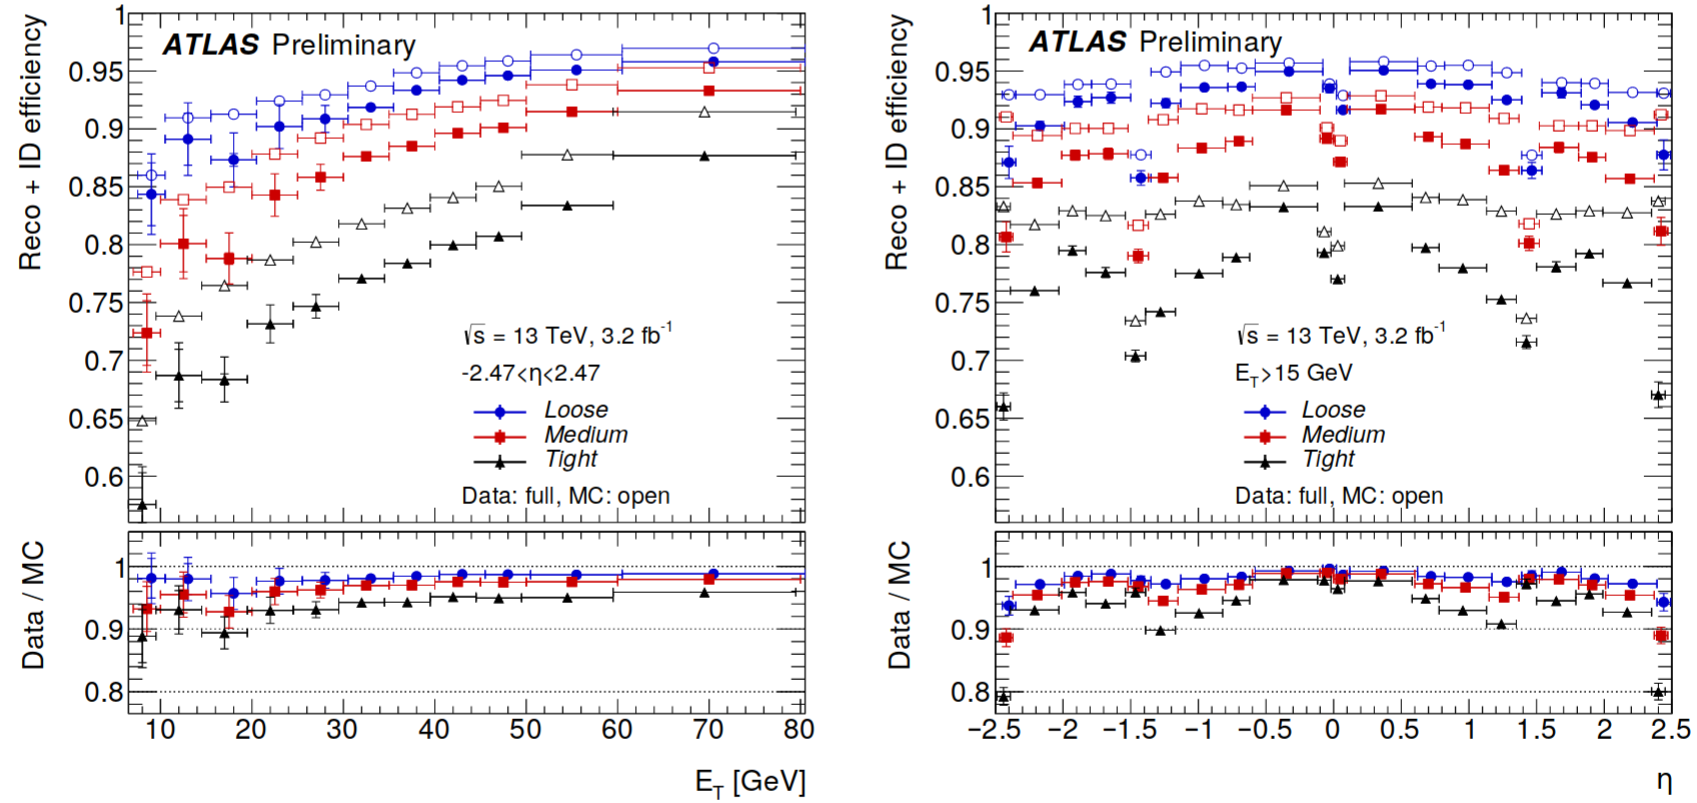
\includegraphics[width=0.9\textwidth]{./figures/object_selection/el_id_eff.png}
        \caption{Combined electron reconstruction and identification efficiencies for $\Z \to \epem$ events as a
                 function of $\et$ (left) and $\eta$ (right) for the \emph{loose}, \emph{medium}, and \emph{tight}
                 working points. The inner error bars show the statistical uncertainty, the outer error bars combine
                 the statistical and systematic uncertainties.~\cite{ATLAS-CONF-2016-024}}\label{fig:object_selection:el_id_eff}
    \end{center}
\end{figure}

\section{Muons}\label{sec:object_selection:muons}

Muons are reconstructed by taking into account information of the inner detector (ID), calorimeter, and the
muon spectrometer (MS).
Because  they traverse the detectors with minimum energy loss, they have a clear signature in the detectors and the
discrimination between them and other physics objects like electrons and jets reaches a high accuracy.

First, muons are reconstructed independently in the ID and the MS\@. The track reconstruction in the ID follows the
usual prescriptions for charged particles~\cite{ATL-SOFT-PUB-2007-007,ATLAS-CONF-2010-072}.
For the track reconstruction in the MS each muon chamber is searched for hit patterns, which are combined to track
segments. The segments are then combined to muon track candidates. For each track candidate a global $\chi^2$ fit
is performed to the hits associated with the track. If a certain threshold is reached the track is accepted~\cite{PERF-2015-10}.

After the individual reconstruction four different algorithms are applied to combine the information of the different
sub-detector systems.
Combined (CB) muons have both a track in the ID and MS\@. The global track is calculated by a refit to both tracks.
If there is only one local track segment in the MDT or CSC chambers and the track of the ID can be extrapolated to the MS
the muon is classified as segment-tagged (ST).
A track in the ID can be classified as calorimeter-tagged (CT) muon if the track can be matched to a energy deposition
in the calorimeter, if it has the signature of a minimum-ionizing particle.
Extrapolated (ME) muons are reconstructed only from tracks in the MS with the additional requirement that the track
needs to originate from the interaction point (IP)\@.

To reduce background from mainly pion and kaon decays, different muon identification criteria are defined.
For \emph{medium} muons only CB and ME tracks are used with some additional requirements on the number of hits in
different layers and the \emph{q/p significance}\footnote{The \emph{q/p significance} is the absolute value of the
difference between charge and momentum measured in ID and MS divided by the sum of squares of the respective uncertainties.}.
In this analysis \emph{loose} muons are used with $\pt > \unit[10]{GeV}$ and $\abs{\eta} < 2.5$.
This includes all \emph{medium} muons as well as CT and ST muons, which are however restricted to $\abs{\eta} < 0.1$.

Isolation requirements can further reduce background, because muons originating from heavy particles like $\W$, $\Z$,
or Higgs bosons are often produced isolated. Two discriminating variables are introduced.
The calorimetric isolation energy $\et^{\text{topocone}20}$ is defined as the sum of transverse energy deposited within
$\dr = 0.2$ around the muon candidates.
Corrections for pile-up and the underlying event activity are applied.
The sum of the transverse momentum of all tracks with $\pt > \unit[1]{GeV}$ within $\dr = \min(0.3, \unit[10]{GeV} / \pt^\mu)$
is defined as the track isolation $\pt^{\text{varcone}0.3}$.
Based on different selections criteria on quantities $\et^{\text{topocone}20} / \pt^\mu$ and
$\pt^{\text{varcone}30} / \pt^\mu$ multiple operating points are constructed.
This analysis uses the \emph{gradient} isolation criterion which provides an efficiency of more than
$\unit[90(99)]{\%}$ at $\unit[20(60)]{GeV}$~\cite{PERF-2015-10}.

The muon reconstruction and identification efficiencies are obtained with a \emph{tag-and-probe technique} using
$\Z \to \mpmm$ and $\JPsi \to \mpmm$ events.
\cref{fig:object_selection:mu_id_eff}\todo{fix vertical label position in figure} shows the reconstruction efficiencies for \emph{medium} and \emph{loose} muons.
The efficiencies are calculated both in data and simulated events in order to derive \emph{scale factors}, which are used
to correct deviations of the efficiencies in data and simulation.

\begin{figure}[!htb]
    \begin{center}
        \begin{subfigure}[c]{0.45\textwidth}
            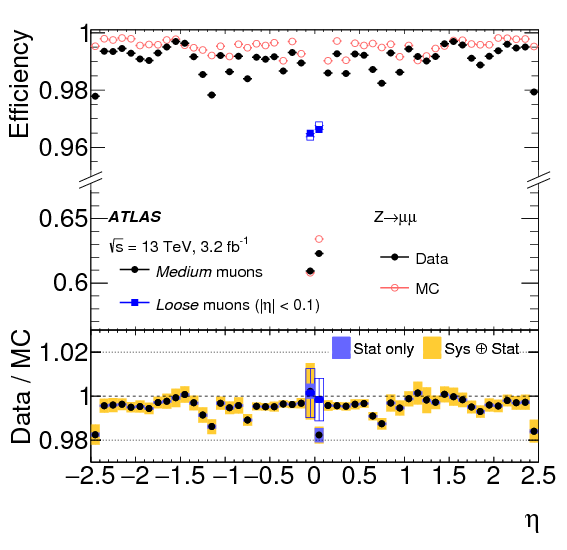
\includegraphics[width=\textwidth]{./figures/object_selection/mu_id_eff_a.png}
            \caption{}
        \end{subfigure}
        \hfill
        \begin{subfigure}[c]{0.45\textwidth}
            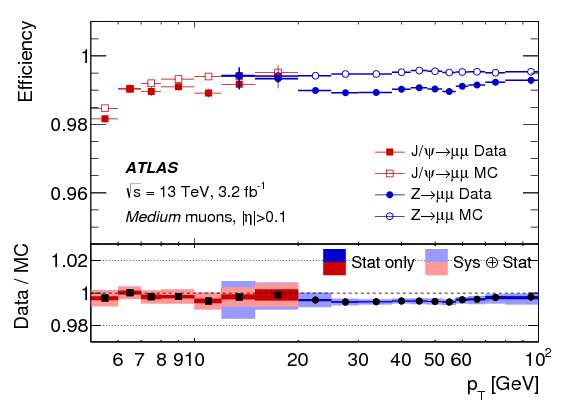
\includegraphics[width=\textwidth]{./figures/object_selection/mu_id_eff_b.png}
            \caption{}
        \end{subfigure}
        \caption{Muon reconstruction efficiencies for \emph{loose} and \emph{medium} muons as a function of $\eta$
                measured in $\Z \to \mpmm$ events (a) and for \emph{medium} muons as a function of $\pt$ measured in
                $\Z \to \mpmm$ and $\JPsi \to \mpmm$ events (b).~\cite{PERF-2015-10}}\label{fig:object_selection:mu_id_eff}
    \end{center}
\end{figure}


\section{Jets}\label{sec:object_selection:jets}

Particles with a color charge like quarks and gluons cannot exist in an unbound state,
they form colorless states due to hadronization.\todo{Ref.\ to theory chapter}
With higher energies of the initial quark or gluon more and more collimated bunches of hadrons are produced.
Those bunches are called \emph{jets}.

An algorithm which reconstructs jets should be insensitive to soft radiation (\emph{infrared safety})
and splitting of the initial seed (\emph{collinear safety}).
There are two types of jet reconstruction algorithms, cone type and sequential clustering algorithms.
Cone type algorithms use a geometrical cone around a jet axis to reconstruct the jet. In the past not
all cone algorithms were infrared and collinear safe.
Sequential cluster algorithms combine different object based on their energy and angular properties.
They provide infrared and collinear safety by construction.

In this analysis the \antikt{}~\cite{Cacciari:2008gp,Cacciari:2005hq} clustering algorithm with a distance parameter
of $R = 0.4$ was used for jet reconstruction.
Not all jets are considered in the analysis, only jets with $\pt > \unit[20]{GeV}$ and $\abs{\eta} < 4.5$ are used.

The jet four-momenta undergo a series of corrections~\cite{PERF-2016-04}, to take several insufficiencies into account.
First, the jet origin is corrected to point back to the primary vertex. Next excess energy due to pile-up is removed.
Truth information of simulated dijet events is used to correct the jet energy scale (JES).
Additional JES corrections are performed in the \emph{global sequential calibration}, which uses calorimeter, muon
spectrometer and track-based variables. Finally an \emph{in-situ} correction in data is applied, using events
in \todo{convention jets/dijet in process description?}$\Z+jets$, $\gamma + jets$, and dijet processes.
These corrections raise a list of systematic uncertainties, which are discussed in \cref{cha:systematic_uncertainties}.\todo{Possibly fix ref to section}

\emph{Pile-up} jets can be suppressed with the output of the jet vertex tagger (JVT) algorithm~\cite{PERF-2014-03}, which
uses tracking and vertexing information to distinguish jets from hard- and soft-scatter interactions.
All jets in this analysis with $\pt < \unit[50]{GeV}$ and $\abs{\eta} < 2.4$ are required to have $\abs{\text{JVT}} > 0.59$.
In the forward region a special algorithm for forward jets (fJVT) is used~\cite{ATL-PHYS-PUB-2015-034}.
For this analysis jets with $\pt < \unit[50]{GeV}$ and $\abs{\eta} > 2.5$ need to pass the fJVT algorithm with
$\text{fJVT} > 0.4$.
\\[\baselineskip]
Since this analysis focus is on the gluon fusion and VBF production modes of the Higgs boson, jets produced from
the decay of a $b$ quark are not expected. However, top quarks have a very high probability of decaying into $b$ quarks,
since the corresponding entry in the CKM matrix is $\abs{V_{tb}} \approx 1$~\cite{PDG}.
This gives the possibility to reduce the background produced by top quarks.

Jets originating from $b$ quarks, also called $b$-jets, can be identified with $b$-tagging algorithms.
These algorithms exploit the fact that $b$-flavoured hadrons (B hadrons) have quite a long mean life time
($\tau \approx \unit[1.5]{ps}$~\cite{PDG}) compared to other hadrons.
The decay creates a secondary vertex several millimeters away from the primary vertex due to time
dilation.\footnote{If a lifetime of $\tau = \unit[1.5]{ps}$ and rest mass of $m_0 = \unit[5.3]{GeV}$ are assumed (approximate values, taken from~\cite{PDG}),
the B hadron travels $c\tau' = c \tau \gamma = c \tau \frac{E}{m_0} = \unit[4.24]{mm}$, if it has an energy of $E = \unit[50]{GeV}$.}.
The secondary vertex is reconstructed with the tracks of the charged particles which formed the jet.

This analysis uses the multivariate-based $b$-tagging algorithm MV2c20~\cite{PERF-2012-04,ATL-PHYS-PUB-2016-012} with
a working point resulting in \unit[85]{\%} efficiency for $b$-jets in $t\overline{t}$ events. In several simulated processes
the comparison to data is used to calculate tagging and mis-tagging correction factors.
The requirements of $\pt > \unit[25]{GeV}$ and $\abs{\eta} < 2.4$ are additionally applied to the $b$-tagged jets.

\section{Missing Transverse Energy}\label{sec:object_selection:missing_transverse_energy}

\section{Tau Leptons}\label{sec:object_selection:tau_leptons}

\section{Overlap Removal}\label{sec:object_selection:overlap_removal}


